
\section{Permanentmagnet-erregte Synchronmaschine (PSM)}

Im Zuge des zweiten Teils der Laborübung erfolgte die Demonstration verschiedener Versuche auf Basis mehrerer Regelprinzipien an einem PSM-Aufbau. Dabei wurde die PSM entsprechend Abbildung \ref{fig:umrichter} über einen Spannungszwischenkreisumrichter versorgt und war mechanisch mit einer Asynchronmaschine gekoppelt. Die Nenndaten beider Maschinen sowie weiterführende Details zum Aufbau sind dem Vorbereitungsskript zu entnehmen.

\begin{figure}[h!]
    \centering
    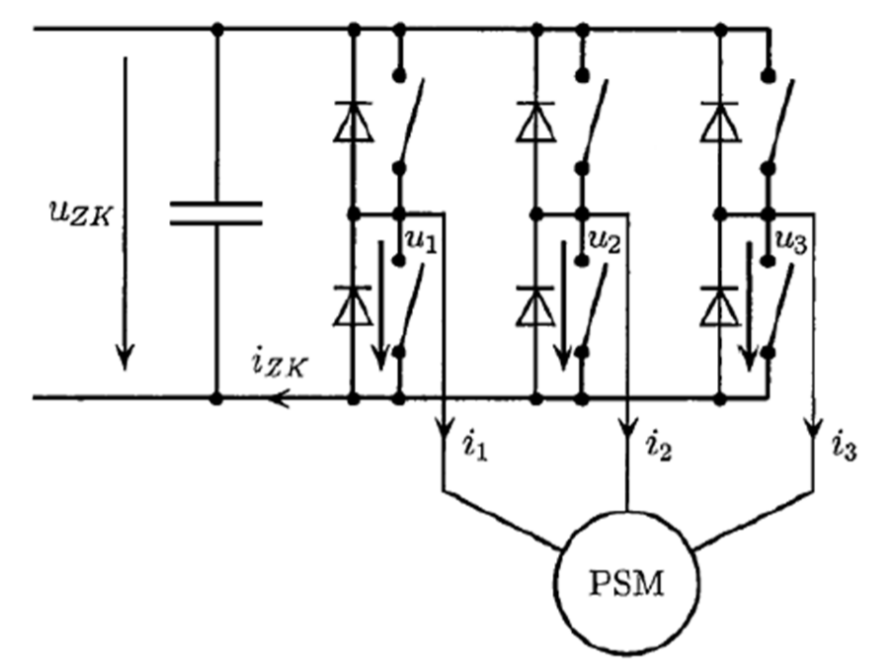
\includegraphics[scale=0.4]{1/Umrichter.png}
    \caption{Verwendeter Spannungszwischenkreisumrichter.}
    \label{fig:umrichter}
\end{figure}

\noindent Der Umrichter inklusive Regeleinheit ermöglicht sowohl BLDC- als auch Feldschwächbetrieb und eine feldorientierte Regelung. Entsprechende Sensoren zeichnen dabei die relevanten Größen auf, welche am Oszilloskop dargestellt und untersucht werden. Im Folgenden wird näher auf die einzelnen Betriebsarten und ihre Messgrößen eingegangen.

\subsection{Feldorientierte Regelung}

\begin{figure}[h!]
    \centering
    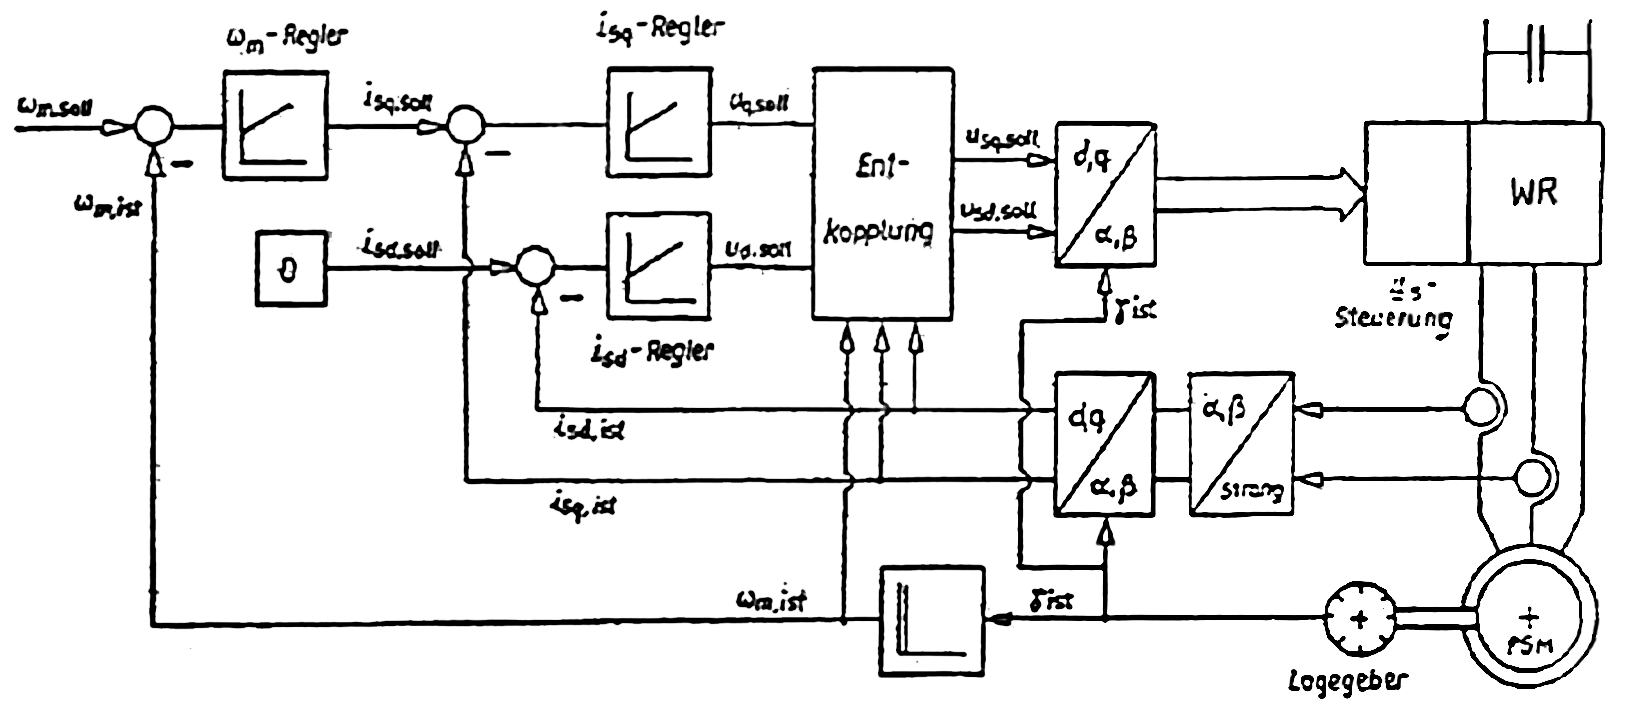
\includegraphics[scale=0.4]{1/Regelung.png}
    \caption{Blockschaltbild einer kaskadierten Regelung mit Entkopplungsnetzwerk.}
    \label{fig:regelkreis}
\end{figure}

\noindent Zunächst wird die hochdynamische feldorientierte Regelung betrachtet, bei der die Drehzahl der Maschine durch das Drehmoment, das entsteht, wenn eine auf den Fluss normal stehende q-Komponente des Stromes eingeprägt wird, beeinflusst werden kann:

\begin{equation}
    m_R=-\operatorname{Im}(\underline{i}_S^* \cdot \underline{\Psi}_S)= i_{S,q} \cdot |\Psi_M|.
\end{equation}

\noindent Der Drehzahl-Regelkreis ist dabei entsprechend Abbildung \ref{fig:regelkreis} dem Stromregler überlagert (zusätzlich kann theoretisch noch eine Lageregelung überlagert werden). Die Entkopplung sorgt dabei für eine Unabhängigkeit der Spannungen $u_d$ und $u_q$ von den jeweiligen Strömen mit gegenteiligem Index. Die d-Komponente des Stromes wird in dieser Betriebsart zu 0 gewählt, da sie keinen Anteil am Drehmoment hat und lediglich zu unerwünschten Kupferverlusten führen würde.\\
\noindent Der erste Versuch ist das Hochlaufen der Maschine aus dem Stillstand - zunächst mit einer Stellgrößenbeschränkung, die lediglich halbes Nennmoment zulässt (Abbildung \ref{fig:hochlauf_halb_dq}), und anschließend ohne Beschränkung (Abbildung \ref{fig:hochlauf_ganz_dq}). Deutlich erkennbar ist der lineare Anstieg der Drehzahl mit der Zeit, sobald die q-Stromkomponente und damit ein Drehmoment wirksam wird, was auf den Drallsatz zurückzuführen ist. Dementsprechend steigt der Lagewinkel als Integral über der Drehzahl quadratisch an. Ein weiterer linearer Zusammenhang ist erkennbar, wenn man die Zeit vergleicht, die jeweils benötigt wird, um die Nenndrehzahl zu erreichen: Im ersten Fall mit Stellgrößenbeschränkung auf halben Strom dauert es auch doppelt so lange ($\approx 300 \si{\milli\second}$) als im Fall ohne Beschränkung ($\approx 150 \si{\milli\second}$). Sobald die gewünschte Drehzahl erreicht ist, sinkt der Strom auf den vergleichsweise geringen Betrag, der dann nur mehr notwendig ist, um die laufenden (Reib-)Verluste abzudecken. Die d-Komponente des Stromes ist dabei, wie gewünscht und erwartet, (bis auf einen gewissen ?Rippel? (Ursache?)) immer verschwindend groß.\\
\noindent In Abbildung \ref{fig:hochlauf_alpha_beta} sind die um $90\degree$ phasenverschobenen Ströme des Hochlaufs im statorfesten $\alpha,\beta$-KOS ersichtlich. Eine Umrechnung dieser gemessenen Stromkomponenten entsprechend

\begin{equation}
    \underline{i}_{S} = i_{\alpha} + j i_{\beta}, \quad i_1=\operatorname{Re}(\underline{i}_{S})=i_{\alpha}, \quad i_2=\operatorname{Re}(\underline{i}_{S} \mathrm{e}^{-j 120 \degree}), \quad i_3=\operatorname{Re}(\underline{i}_{S} \mathrm{e}^{-j 240 \degree})
    \label{eq:umrechnung}
\end{equation}

\noindent in die jeweiligen Phasenströme liefert einen Zeitverlauf gemäß Abbildung \ref{fig:phasenstroeme_feldorientiert} (nicht direkt gemessen). Zu erkennen ist deutlich der sinusförmige Verlauf der um jeweils $120 \degree$ phasenverschobenen Ströme und die mit zunehmender Rotordrehzahl steigende Frequenz. Außerdem addieren sie sich in jedem Zeitpunkt zu 0.\\ 
\noindent Als nächster Versuch zum feldorientierten Betrieb erfolgte ein Drehzahlsprung, dessen Messgrößen in Abbildung \ref{fig:sprung_sinus} ersichtlich sind. Dabei wurde die Maschine ausgehend von $\omega_m=-1$ ohne Stellgrößenbeschränkung auf $\omega_m=1$ in die entgegengesetzte Drehrichtung beschleunigt. Man erkennt beim Start des Vorganges ein bremsendes Moment durch Einprägen einer entsprechenden q-Stromkomponente. Die Drehzahl sinkt, bis sie 0 erreicht, und steigt anschließend aufgrund des wirkenden Momentes zur Folge des eingeprägten Stromes wieder in die gewünschte Richtung. Die Maschine beschleunigt wieder auf die gewünschte Drehzahl und es verbleibt abermals lediglich eine geringe Stromkomponente zur Kompensation der laufenden Verluste. Trägt man die Ströme jeweils auf die x- und y-Achse auf, so erhält man entsprechend Abbildung \ref{fig:stromortskurve_feldorientiert} die Stromortskurve für den feldorientierten Betrieb. Ausgehend von einem geringen Strom zur Folge der Reibung wird der Betrag des Stromes erhöht und der Stromraumzeiger vollführt im betrachteten statischen Koordinatensystem mit der Zeit eine annähernd kreisförmige Bewegung. Ist die gewünschte Drehzahl erreicht, verringert sich der Betrag wieder auf jenen Wert, der notwendig ist, um die laufenden Restverluste abzudecken. Die Ortskurve entspricht dabei nicht perfekt einem Kreis, da die diskrete Oberflächenanordnung der Permanentmagnete eine nicht sinusförmige Feldverteilung im Luftspalt hervorruft - daraus resultieren die gemessenen Oberschwingungen als ,,Ecken'' in der $\alpha,\beta$-Stromortskurve. (Stimmt das so? Warum genau, physikalisch?)
\input{\currfiledir hochlauf_halb_dq.tex}
\input{\currfiledir hochlauf_ganz_dq.tex}
\input{\currfiledir hochlauf_alpha_beta.tex}
\input{\currfiledir phasenstroeme.tex}
\input{\currfiledir drehzahlsprung.tex}
\input{\currfiledir stromortskurve.tex}



